\documentclass[aspectratio=169,18pt]{beamer}

% Packages
\usepackage{tikz}
\usetikzlibrary{positioning, arrows.meta, shapes.geometric, shadows.blur, decorations.pathmorphing}
\usepackage{pgfplots}
\pgfplotsset{compat=1.18}
\usepackage{booktabs}
\usepackage{amsmath}
\usepackage{siunitx}
\usepackage{graphicx}
\usepackage{array}
\usepackage{multirow}

% Custom Color Scheme - Aerospace Theme
\definecolor{navydeep}{RGB}{6,90,130}      % Deep ocean blue
\definecolor{navymain}{RGB}{28,114,147}    % Main navy
\definecolor{tealaccent}{RGB}{33,41,92}    % Dark accent
\definecolor{lightblue}{RGB}{202,220,252}  % Light blue
\definecolor{iceblue}{RGB}{232,243,255}    % Very light blue
\definecolor{warmgray}{RGB}{100,100,100}   % Warm gray for text

% Theme Configuration
\usetheme{Madrid}
\usecolortheme{default}
\setbeamertemplate{navigation symbols}{}
\setbeamertemplate{footline}[frame number]

% Custom color settings
\setbeamercolor{palette primary}{bg=navydeep,fg=white}
\setbeamercolor{palette secondary}{bg=navymain,fg=white}
\setbeamercolor{palette tertiary}{bg=tealaccent,fg=white}
\setbeamercolor{palette quaternary}{bg=navymain,fg=white}
\setbeamercolor{structure}{fg=navydeep}
\setbeamercolor{section in toc}{fg=navymain}
\setbeamercolor{frametitle}{bg=navymain,fg=white}
\setbeamercolor{title}{fg=white}
\setbeamercolor{block title}{bg=navymain,fg=white}
\setbeamercolor{block body}{bg=iceblue,fg=black}
\setbeamercolor{itemize item}{fg=navymain}
\setbeamercolor{itemize subitem}{fg=navymain}

% Enhanced bullet points
\setbeamertemplate{itemize items}[circle]
\setbeamertemplate{enumerate items}[circle]

% Title Information
\title{\textbf{Fixed-Wing UAV for Emergency Medical Delivery}}
\subtitle{AS5213: Conceptual Design of UAVs}
\author{DS Vivek \and Divyam Pandey \and G. Vishwas \and Manav Agarwal \and Monisha V \and \\Abhijeet Mangela}
\institute{Group 11: Skunk Works \\ Department of Aerospace Engineering \\ IIT Madras}
\date{April 2026}

\begin{document}

% ============ SLIDE 1: TITLE SLIDE ============
{
\setbeamertemplate{footline}{} % Remove footer from title slide
\setbeamercolor{background canvas}{bg=navydeep}
\begin{frame}
\titlepage
\begin{center}
\vspace{-0.3cm}
\colorbox{white}{\parbox{0.8\textwidth}{\centering\textcolor{navymain}{\textbf{\large [IMAGE PLACEHOLDER: Insert isometric CAD render from report]}}}}
\end{center}
\end{frame}
}

% ============ SLIDE 2: MISSION REQUIREMENTS ============
\begin{frame}{Mission Profile and Requirements (1/2)}

\begin{tikzpicture}[remember picture,overlay]
\fill[lightblue!30] (current page.north west) rectangle ([yshift=-1.2cm]current page.north east);
\end{tikzpicture}

\textbf{\color{navymain}Design Objective:}
\begin{itemize}
\item Fixed-wing UAV for time-critical medical delivery
\item Target: Antivenom and blood products to remote areas
\item Maximum wingspan: \textcolor{navymain}{\textbf{\SI{2.00}{\meter}}}
\item Payload capacity: \textcolor{navymain}{\textbf{\SI{1.00}{\kilo\gram}}} (droppable)
\end{itemize}

\vspace{0.3cm}
\textbf{\color{navymain}Key Requirements:}
\begin{itemize}
\item Operational radius: \SIrange{40}{50}{\kilo\meter}
\item Total range: \SIrange{80}{100}{\kilo\meter}
\item Cruise speed: \SIrange{18}{25}{\meter\per\second}
\item STOL capability: Takeoff distance $<$ \SI{150}{\meter}
\item Endurance: \SIrange{1}{2}{\hour}
\end{itemize}
\end{frame}

% ============ SLIDE 3: MISSION PROFILE ============
\begin{frame}{Mission Profile and Requirements (2/2)}

\begin{tikzpicture}[remember picture,overlay]
\fill[lightblue!30] (current page.north west) rectangle ([yshift=-1.2cm]current page.north east);
\end{tikzpicture}

\begin{columns}[T]
\column{0.4\textwidth}
\textbf{\color{navymain}Mission Phases:}
\begin{enumerate}
\item Takeoff (STOL)
\item Climb to cruise altitude
\item Cruise (outbound)
\item \textcolor{navydeep}{\textbf{Payload drop without landing}}
\item Turn/Loiter
\item \textcolor{navydeep}{\textbf{Re-climb phase}}
\item Cruise (inbound)
\item Descent and landing
\end{enumerate}

\column{0.55\textwidth}
\begin{center}
% \colorbox{iceblue}{\parbox{0.9\textwidth}{\centering\textcolor{navymain}{\textbf{[IMAGE PLACEHOLDER:\\ Insert Mission Profile diagram\\ from report page 6]}}}}
\begin{figure}
    \centering
    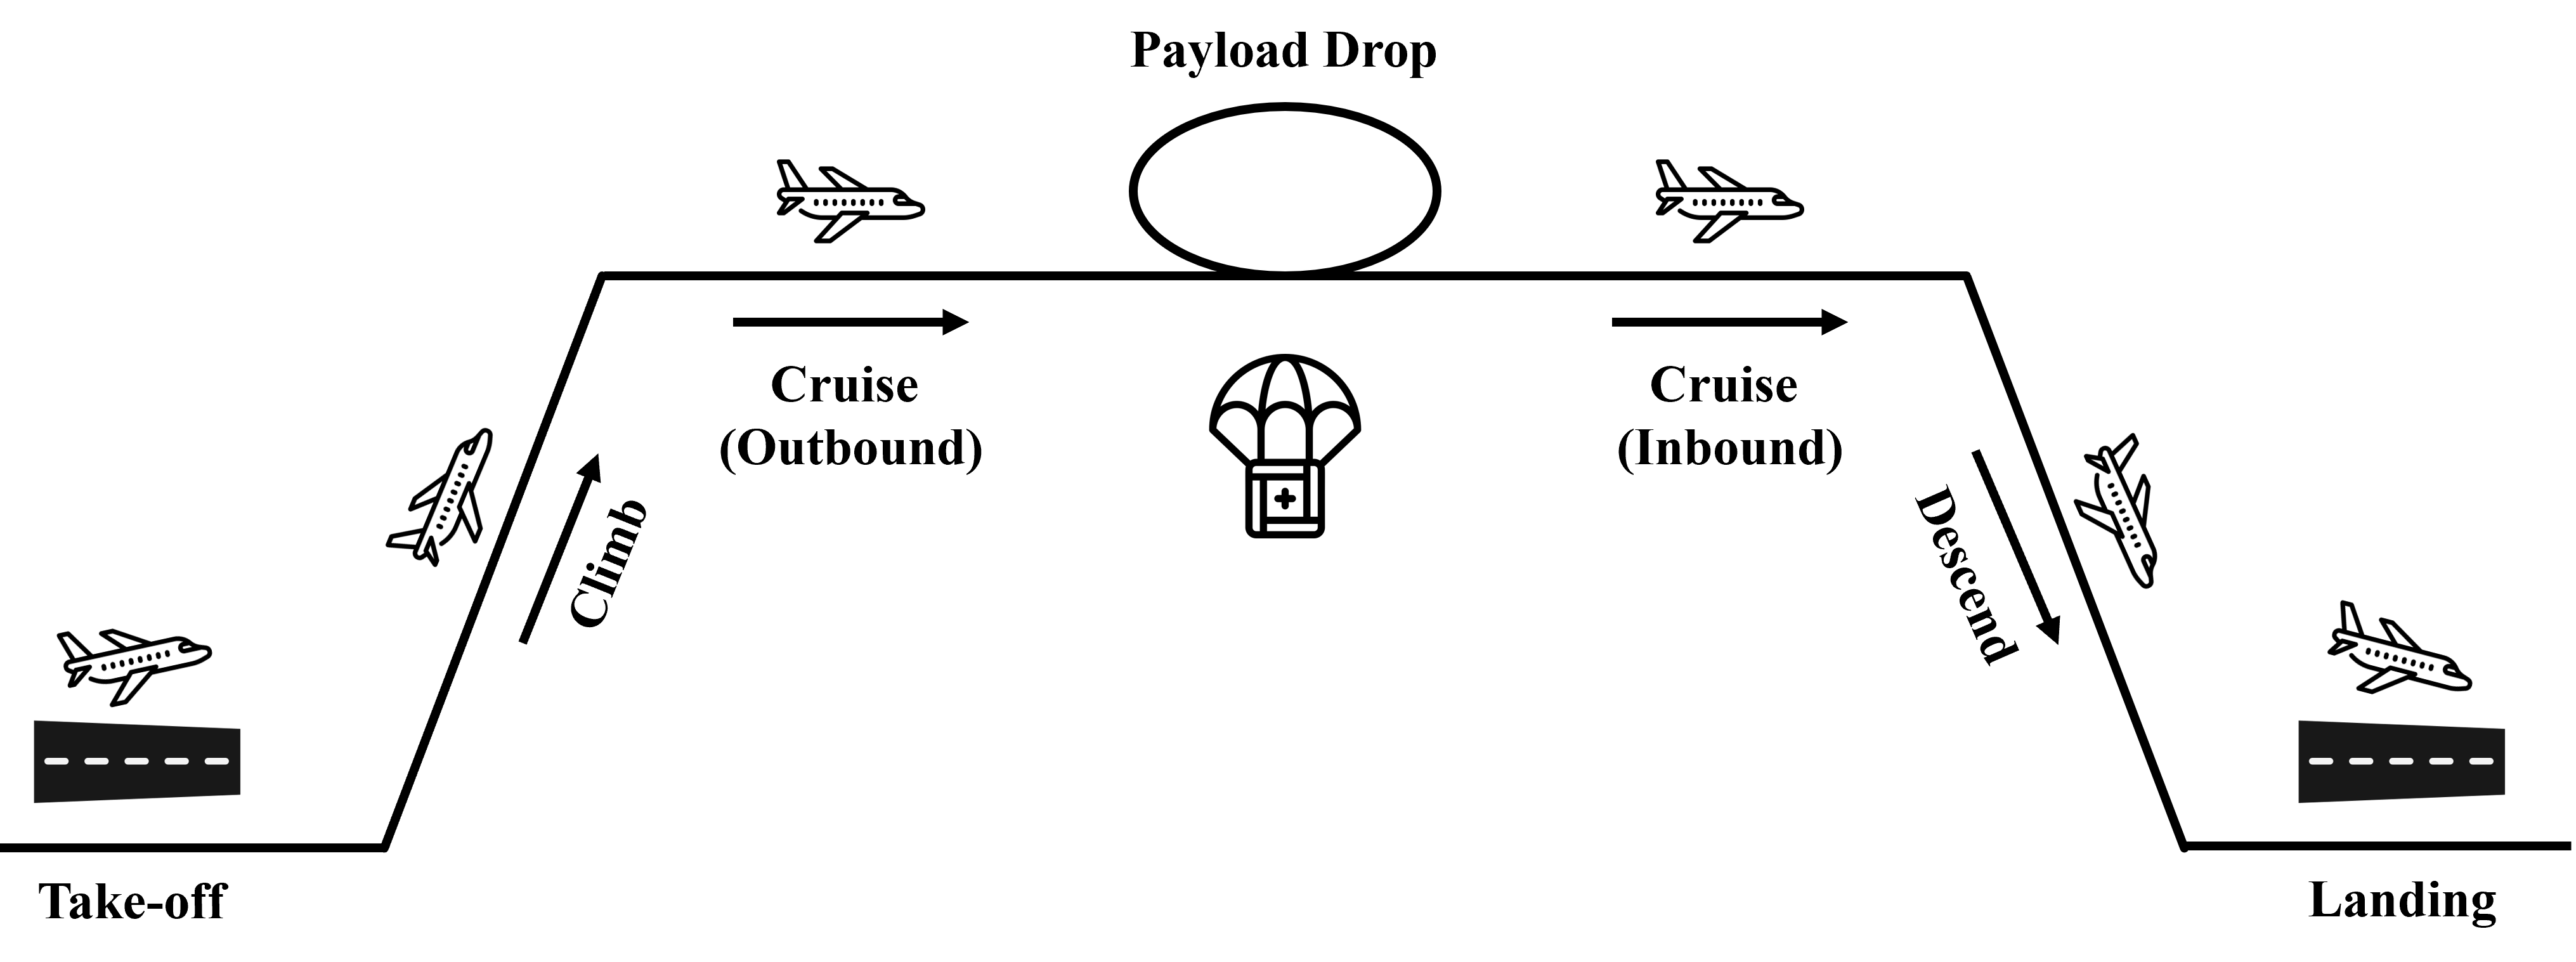
\includegraphics[width=\linewidth]{Mission Profile_new.png}
    \caption{Mission Profile of UAV}
    \label{fig:placeholder}
\end{figure}
\end{center}
\end{columns}
\end{frame}

% ============ SLIDE 4: DESIGN FLOWCHART ============
\begin{frame}{Design Methodology}
\vspace{-0.3cm}
\begin{center}
\resizebox{0.95\textwidth}{!}{%
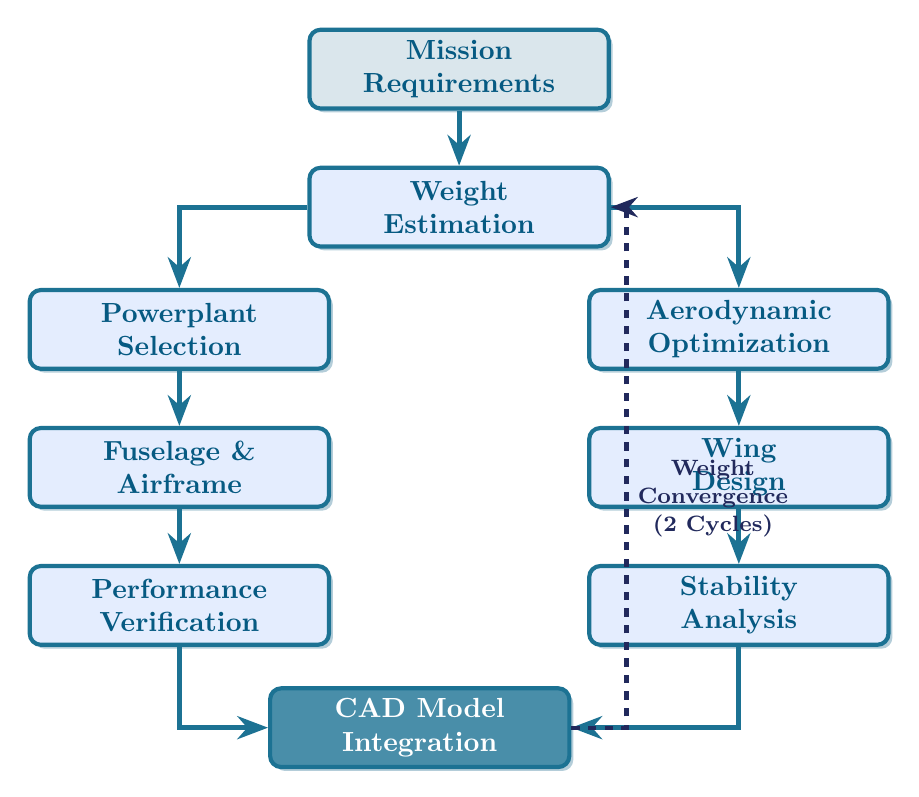
\begin{tikzpicture}[
    node distance=0.7cm and 1.2cm,
    box/.style={
        rectangle, 
        draw=navymain, 
        rounded corners=4pt, 
        line width=1.5pt,
        minimum width=3.8cm, 
        minimum height=1.0cm, 
        align=center,
        fill=white,
        drop shadow={shadow xshift=0.5mm, shadow yshift=-0.5mm, opacity=0.3, fill=navydeep},
        font=\fontsize{10}{12}\selectfont\bfseries
    },
    boxstart/.style={
        box,
        fill=navydeep!15,
        text=navydeep
    },
    boxprocess/.style={
        box,
        fill=lightblue!50,
        text=navydeep
    },
    boxend/.style={
        box,
        fill=navymain!80,
        text=white
    },
    arrow/.style={
        ->,
        line width=1.8pt,
        >=Stealth,
        color=navymain
    },
    arrowback/.style={
        ->,
        line width=1.5pt,
        >=Stealth,
        color=tealaccent,
        dashed
    }
]

% Nodes
\node[boxstart] (req) {Mission\\Requirements};
\node[boxprocess, below=of req] (weight) {Weight\\Estimation};
\node[boxprocess, below left=0.5cm and -0.3cm of weight] (power) {Powerplant\\Selection};
\node[boxprocess, below right=0.5cm and -0.3cm of weight] (aero) {Aerodynamic\\Optimization};
\node[boxprocess, below=of power] (fuse) {Fuselage \&\\Airframe};
\node[boxprocess, below=of aero] (wing) {Wing\\Design};
\node[boxprocess, below=of fuse] (perf) {Performance\\Verification};
\node[boxprocess, below=of wing] (stab) {Stability\\Analysis};
\node[boxend, below right=0.5cm and -0.8cm of perf] (cad) {CAD Model\\Integration};

% Main flow arrows
\draw[arrow] (req) -- (weight);
\draw[arrow] (weight) -| (power);
\draw[arrow] (weight) -| (aero);
\draw[arrow] (power) -- (fuse);
\draw[arrow] (aero) -- (wing);
\draw[arrow] (fuse) -- (perf);
\draw[arrow] (wing) -- (stab);
\draw[arrow] (perf) |- (cad);
\draw[arrow] (stab) |- (cad);

% Feedback Loop (FIXED: added align=center so \\ works)
\draw[arrowback] (cad.east) -- ++(0.7,0) |- node[pos=0.22, right, align=center, font=\fontsize{8}{10}\selectfont\bfseries, text=tealaccent] {Weight\\Convergence\\(2 Cycles)} (weight.east);

\end{tikzpicture}%
}
\end{center}
\end{frame}

% ============ SLIDE 5: POWERPLANT 1 ============
\begin{frame}{Powerplant Specifications (1/2)}



\begin{columns}[T]
\column{0.5\textwidth}
\begin{figure}
    \centering
    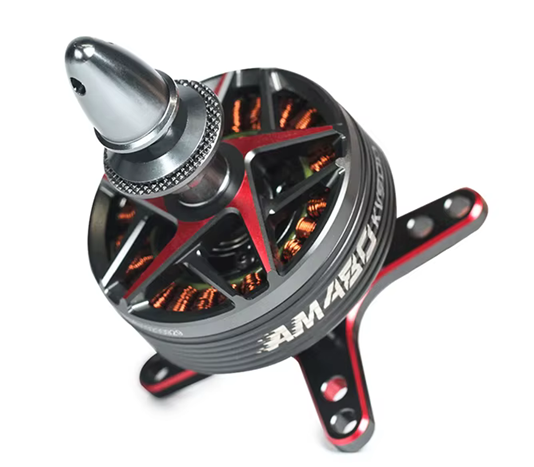
\includegraphics[width=0.5\linewidth]{TMotor.png}
    \caption{T-Motor AM480 900KV}
    \label{fig:placeholder}
\end{figure}
\textbf{\color{navymain}Motor Selection:}
\begin{itemize}
\item \textbf{Model:} T-Motor AM480 900KV
\item \textbf{Configuration:} Dual-motor tractor
\item \textbf{Max Power:} \textcolor{navydeep}{\SI{450}{\watt}} at 80 $\%$ Throttle
\item \textbf{Voltage:} \SI{11.1}{\volt} (3S LiPo)
\item \textbf{Peak Current:} \SI{26}{\ampere}
\item \textbf{ESC:} Hobbywing Skywalker 50A V2
\end{itemize}

\column{0.5\textwidth}
\begin{figure}
    \centering
    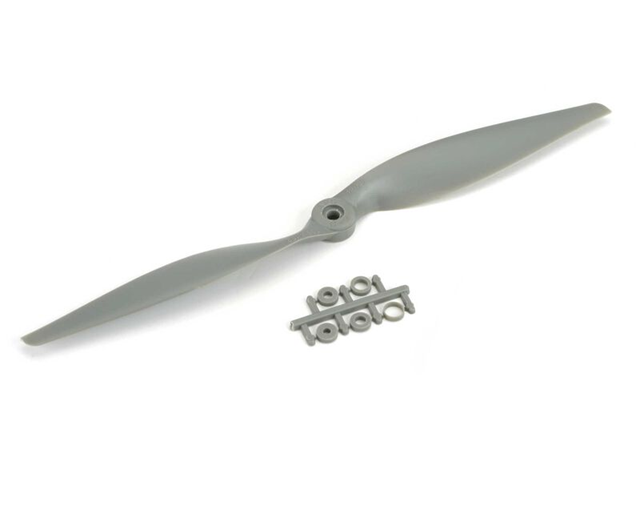
\includegraphics[width=0.5\linewidth]{prp.png}
    \caption{Propellor}
    \label{fig:placeholder}
\end{figure}
\textbf{\color{navymain}Propeller:}
\begin{itemize}
\item \textbf{Model:} APC 12$\times$6E (electric)
\item \textbf{Diameter:} 12~in (\SI{0.305}{\meter})
\item \textbf{Pitch:} 6~in
\item \textbf{Cruise efficiency:} Optimized for \SIrange{300}{350}{\watt}
\end{itemize}
\end{columns}

\vspace{0.5cm}
\begin{center}

\begin{tikzpicture}
\fill[navymain!20, rounded corners=3pt] (0,0) rectangle (10,0.8);
\node[anchor=west] at (0.3,0.4) {\textbf{\color{navydeep}Configuration:} Dual tractor motors on wing leading edge};
\end{tikzpicture}
\end{center}
\end{frame}


% ============ SLIDE 6: POWERPLANT 2 ============
\begin{frame}{Powerplant Specifications (2/2)}


\begin{columns}[T]


\column{0.5\textwidth}
\textbf{\color{navymain}Battery System:}
\begin{figure}
    \centering
    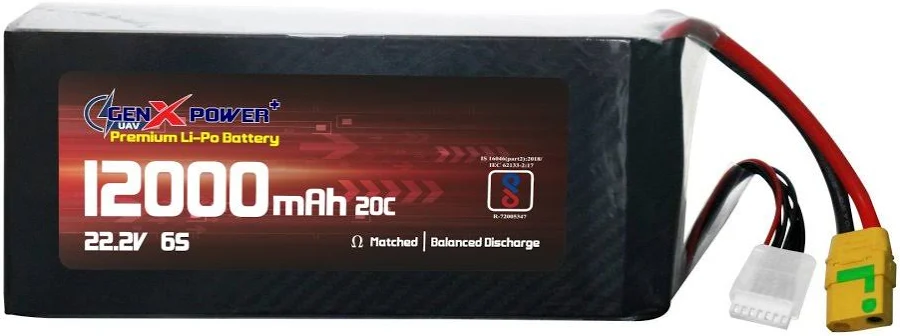
\includegraphics[width=0.5\linewidth]{genx_battery.png}
    \caption{Caption}
    \label{fig:placeholder}
\end{figure}
\begin{itemize}
\item \textbf{Model:} GenX 6S \SI{12}{\ampere\hour}
\item \textbf{Voltage:} \SI{22.2}{\volt} nominal
\item \textbf{Capacity:} \SI{12000}{\milli\ampere\hour}
\item \textbf{Mass:} \textcolor{navydeep}{\textbf{\SI{1524}{\gram}}}
\item \textbf{Dimensions:} $183 \times 75 \times 34$ mm
\item \textbf{Total energy:} \SI{959}{\kilo\joule}
\end{itemize}

\column{0.5\textwidth}
\textbf{\color{navymain}Power Budget:}
\begin{itemize}
\item Peak power (climb): \textcolor{navydeep}{\textbf{\SI{361.46}{\watt}}}
\item Required thrust: \SI{14.73}{\newton}
\item Avionics: \SI{6.61}{\watt} total
\item Battery efficiency: \textcolor{navydeep}{\textbf{85\%}}
\item Motor efficiency: \textcolor{navydeep}{\textbf{82\%}}
\end{itemize}
\end{columns}
\end{frame}

% ============ SLIDE 7: AERODYNAMICS 1 ============
\begin{frame}{Aerodynamic Parameters (1/2)}

\begin{tikzpicture}[remember picture,overlay]
\fill[lightblue!30] (current page.north west) rectangle ([yshift=-1.2cm]current page.north east);
\end{tikzpicture}

\begin{columns}[T]
\column{0.5\textwidth}
\textbf{\color{navymain}Wing Configuration:}
\begin{itemize}
\item \textbf{Airfoil:} Selig S7055
\item \textbf{Planform:} Rectangular, high-wing
\item \textbf{Aspect ratio (AR):} \textcolor{navydeep}{\textbf{7.53}}
\item \textbf{Wing area ($S$):} \SI{0.5307}{\meter\squared}
\item \textbf{Wingspan ($b$):} \textcolor{navydeep}{\textbf{\SI{2.00}{\meter}}}
\item \textbf{Mean chord ($\bar{c}$):} \SI{0.2653}{\meter}
\item \textbf{Taper ratio:} 1.0 (rectangular)
\end{itemize}

\column{0.5\textwidth}

\textbf{\color{navymain}Drag Polar:}
\begin{itemize}
\item \textbf{Zero-lift drag:} $C_{D_0} = 0.02873$
\item \textbf{Induced drag factor ($k$):} $\frac{1}{\pi e \cdot AR}$
\item \textbf{Oswald efficiency:} $e = 0.85$
\end{itemize}

\vspace{0.5cm}
\begin{center}

\begin{tikzpicture}
\fill[navydeep, rounded corners=3pt] (0,0) rectangle (4.5,1.2);
\node[text=white, align=center] at (2.25,0.6) {\textbf{Max L/D Ratio}\\\LARGE\textbf{12.55}};
\end{tikzpicture}
\end{center}
\end{columns}
\end{frame}

% ============ SLIDE 8: AERODYNAMICS 2 ============
\begin{frame}{Aerodynamic Parameters (2/2)}


\begin{columns}[T]
\column{0.5\textwidth}
\textbf{\color{navymain}Lift Characteristics:}
\begin{itemize}
\item \textbf{Max L/D ratio:} 12.55 (at cruise)
\item \textbf{$C_{L,\text{cruise}}$:} 0.65--0.75
\item \textbf{$C_{L,\text{max}}$:} \textcolor{navydeep}{\textbf{1.4}}
\item \textbf{Lift-curve slope:} $C_{L_\alpha} = \SI{5.73}{\per\radian}$
\item \textbf{Stall speed:} \textcolor{navydeep}{\textbf{\SI{12.4}{\meter\per\second}}}
\end{itemize}

\column{0.5\textwidth}
\begin{center}
\begin{figure}
    \centering
    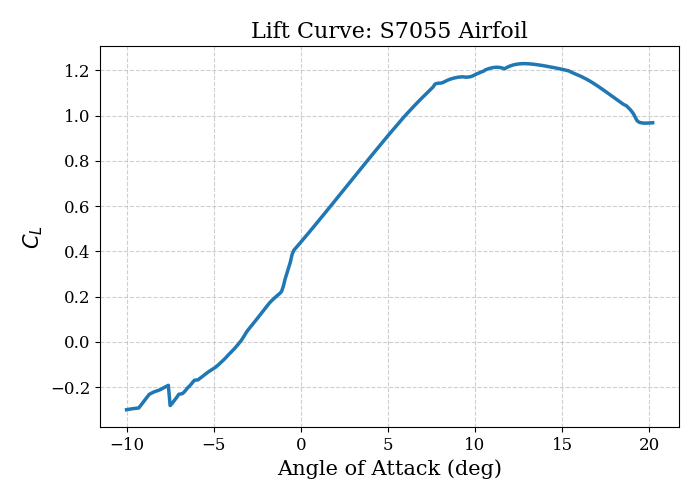
\includegraphics[width=0.5\linewidth]{cl_alp.png}
    \caption{Caption}
    \label{fig:placeholder}
\end{figure}

\vspace{0.5cm}
\begin{figure}
    \centering
    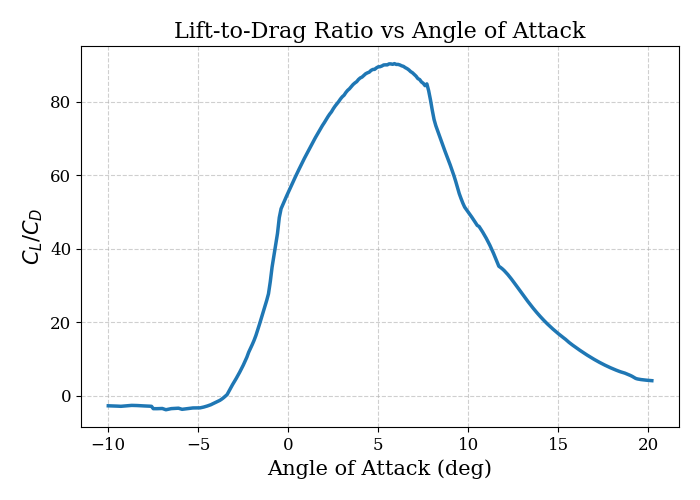
\includegraphics[width=0.5\linewidth]{CL_Cd_alpha.png}
    \caption{Caption}
    \label{fig:placeholder}
\end{figure}
\end{center}
\end{columns}
\end{frame}

% ============ SLIDE 9: INERTIA AND GEOMETRY 1 ============
\begin{frame}{Inertia and Geometric Parameters (1/2)}

\begin{columns}[T]
\column{0.5\textwidth}
\textbf{\color{navymain}Mass Properties:}
\begin{itemize}
\item \textbf{MTOW:} \textcolor{navydeep}{\textbf{\SI{6.59}{\kilo\gram}}}
\item \textbf{Empty weight:} \SI{3.29}{\kilo\gram}
\item \textbf{Battery:} \SI{0.987}{\kilo\gram}
\item \textbf{Payload:} \SI{1.20}{\kilo\gram} (droppable)
\item \textbf{Avionics:} \SI{0.90}{\kilo\gram}
\item \textbf{Empty weight fraction:} 0.50
\end{itemize}

\column{0.5\textwidth}
\textbf{\color{navymain}Center of Gravity:}
\begin{itemize}
\item \textbf{Longitudinal CG:} \SI{264}{\milli\meter} from nose
\item \textbf{Lateral CG:} \SI{0}{\milli\meter} (symmetric)
\item \textbf{Static margin:} \textcolor{navydeep}{\textbf{$\approx 14\%$ MAC}}
\end{itemize}
\end{columns}

\vspace{0.5cm}
\begin{center}
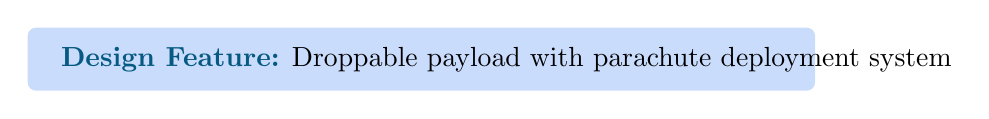
\begin{tikzpicture}
\fill[lightblue, rounded corners=3pt] (0,0) rectangle (10,0.8);
\node[anchor=west] at (0.3,0.4) {\textbf{\color{navydeep}Design Feature:} Droppable payload with parachute deployment system};
\end{tikzpicture}
\end{center}
\end{frame}

% ============ SLIDE 10: INERTIA AND GEOMETRY 2 ============
\begin{frame}{Inertia and Geometric Parameters (2/2)}

\begin{tikzpicture}[remember picture,overlay]
\fill[lightblue!30] (current page.north west) rectangle ([yshift=-1.2cm]current page.north east);
\end{tikzpicture}

\textbf{\color{navymain}Fuselage Dimensions:}
\begin{itemize}
\item \textbf{Total length:} \SI{1.10}{\meter}
\item \textbf{Fuselage diameter:} \SI{0.15}{\meter}
\item \textbf{Tail boom length:} \SI{0.70}{\meter}
\end{itemize}

\vspace{0.3cm}
\textbf{\color{navymain}Empennage \& Control:}
\begin{itemize}
\item \textbf{Horizontal tail area:} $S_t = \SI{0.133}{\meter\squared}$ \quad \textbf{Span:} \SI{0.773}{\meter}
\item \textbf{Tail arm:} $l_t = \SI{0.70}{\meter}$ \quad \textbf{Airfoil:} NACA 0012
\item \textbf{Tail setting angle:} $i_t = -0.31^\circ$
\item \textbf{Vertical tail area:} $S_v = \SI{0.080}{\meter\squared}$
\item \textbf{Control Surfaces:} Elevator, rudder, ailerons
\item \textbf{Deflection limits:} $-15^\circ$ to $+25^\circ$ (elevator)
\end{itemize}
\end{frame}

% ============ SLIDE 11: PERFORMANCE 1 ============
\begin{frame}{Performance Parameters (1/2)}


\begin{columns}[T]
\column{0.5\textwidth}
\textbf{\color{navymain}Flight Envelope:}
\begin{itemize}
\item \textbf{Maximum range:} \textcolor{navydeep}{\textbf{\SI{83.15}{\kilo\meter}}}
\item \textbf{Endurance:} \textcolor{navydeep}{\textbf{2 h 5 min}}
\item \textbf{Cruise speed:} \SIrange{18}{22}{\meter\per\second}
\item \textbf{Stall speed:} \SI{12.4}{\meter\per\second}
\item \textbf{Maximum speed:} \SI{28}{\meter\per\second}
\item \textbf{Service ceiling:} \SI{2000}{\meter}

\begin{figure}
    \centering
    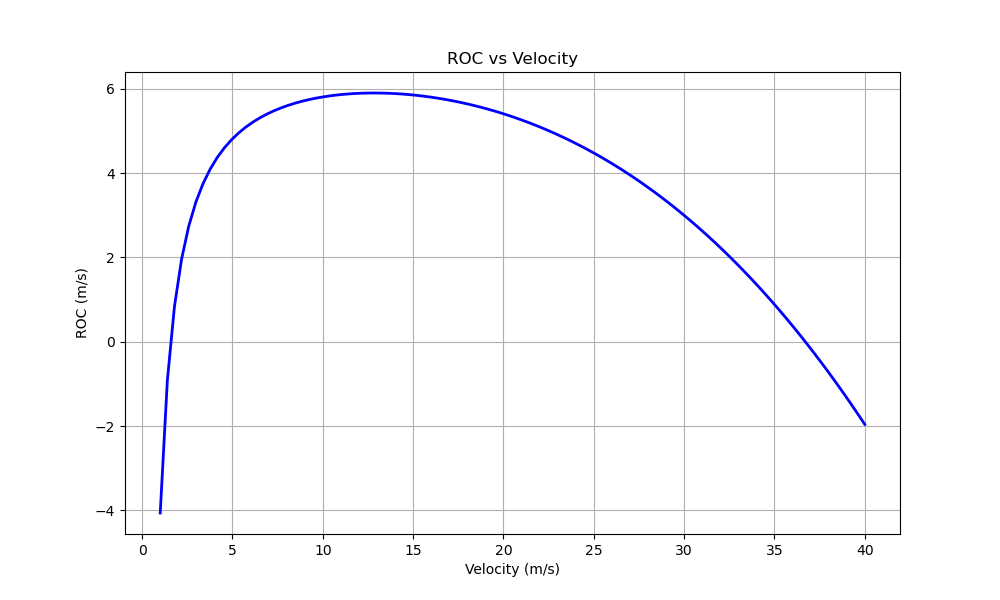
\includegraphics[width=0.5\linewidth]{ROC_vs_Velocity.png}
    \caption{Rate of climb vs velocity}
    \label{fig:placeholder}
\end{figure}
\end{itemize}

\column{0.5\textwidth}
\textbf{\color{navymain}Climb Performance:}
\begin{itemize}
\item \textbf{Rate of climb:} \textcolor{navydeep}{\textbf{\SI{3.5}{\meter\per\second}}}
\item \textbf{Climb angle:} $15^\circ$--$20^\circ$
\item \textbf{Optimal climb speed:} \SI{16}{\meter\per\second}
\end{itemize}

\vspace{0.5cm}
\begin{center}

\begin{tikzpicture}
\fill[navydeep, rounded corners=3pt] (0,0) rectangle (4.5,1.2);
\node[text=white, align=center] at (2.25,0.6) {\textbf{STOL Capability}\\\textbf{Takeoff < 150m}};
\end{tikzpicture}
\end{center}
\end{columns}
\end{frame}

% ============ SLIDE 12: PERFORMANCE 2 ============
\begin{frame}{Performance Parameters (2/2)}


\begin{columns}[T]
\column{0.5\textwidth}
\textbf{\color{navymain}Takeoff/Landing (STOL):}
\begin{itemize}
\item \textbf{Takeoff distance:} $< \SI{150}{\meter}$
\item \textbf{Liftoff velocity:} \SI{13.6}{\meter\per\second}
\item \textbf{Landing distance:} $< \SI{120}{\meter}$
\item \textbf{Approach speed:} \SI{15}{\meter\per\second}
\end{itemize}

\vspace{0.3cm}
\textbf{\color{navymain}Comparative Performance:}
\begin{table}
\fontsize{11}{13}\selectfont
\begin{tabular}{@{}lcc@{}}
\toprule
\textbf{Parameter} & \textbf{Required} & \textbf{Achieved} \\
\midrule
Range (km) & 80--100 & \textcolor{navydeep}{\textbf{83.15}} \\
Endurance (hr) & 1--2 & \textcolor{navydeep}{\textbf{2.08}} \\
Cruise (m/s) & 18--25 & \textcolor{navydeep}{\textbf{18--22}} \\
Payload (kg) & 1--2 & \textcolor{navydeep}{\textbf{1.20}} \\
\bottomrule
\end{tabular}
\end{table}

\column{0.5\textwidth}
\vspace{0.3cm}
\begin{center}
\begin{figure}
    \centering
    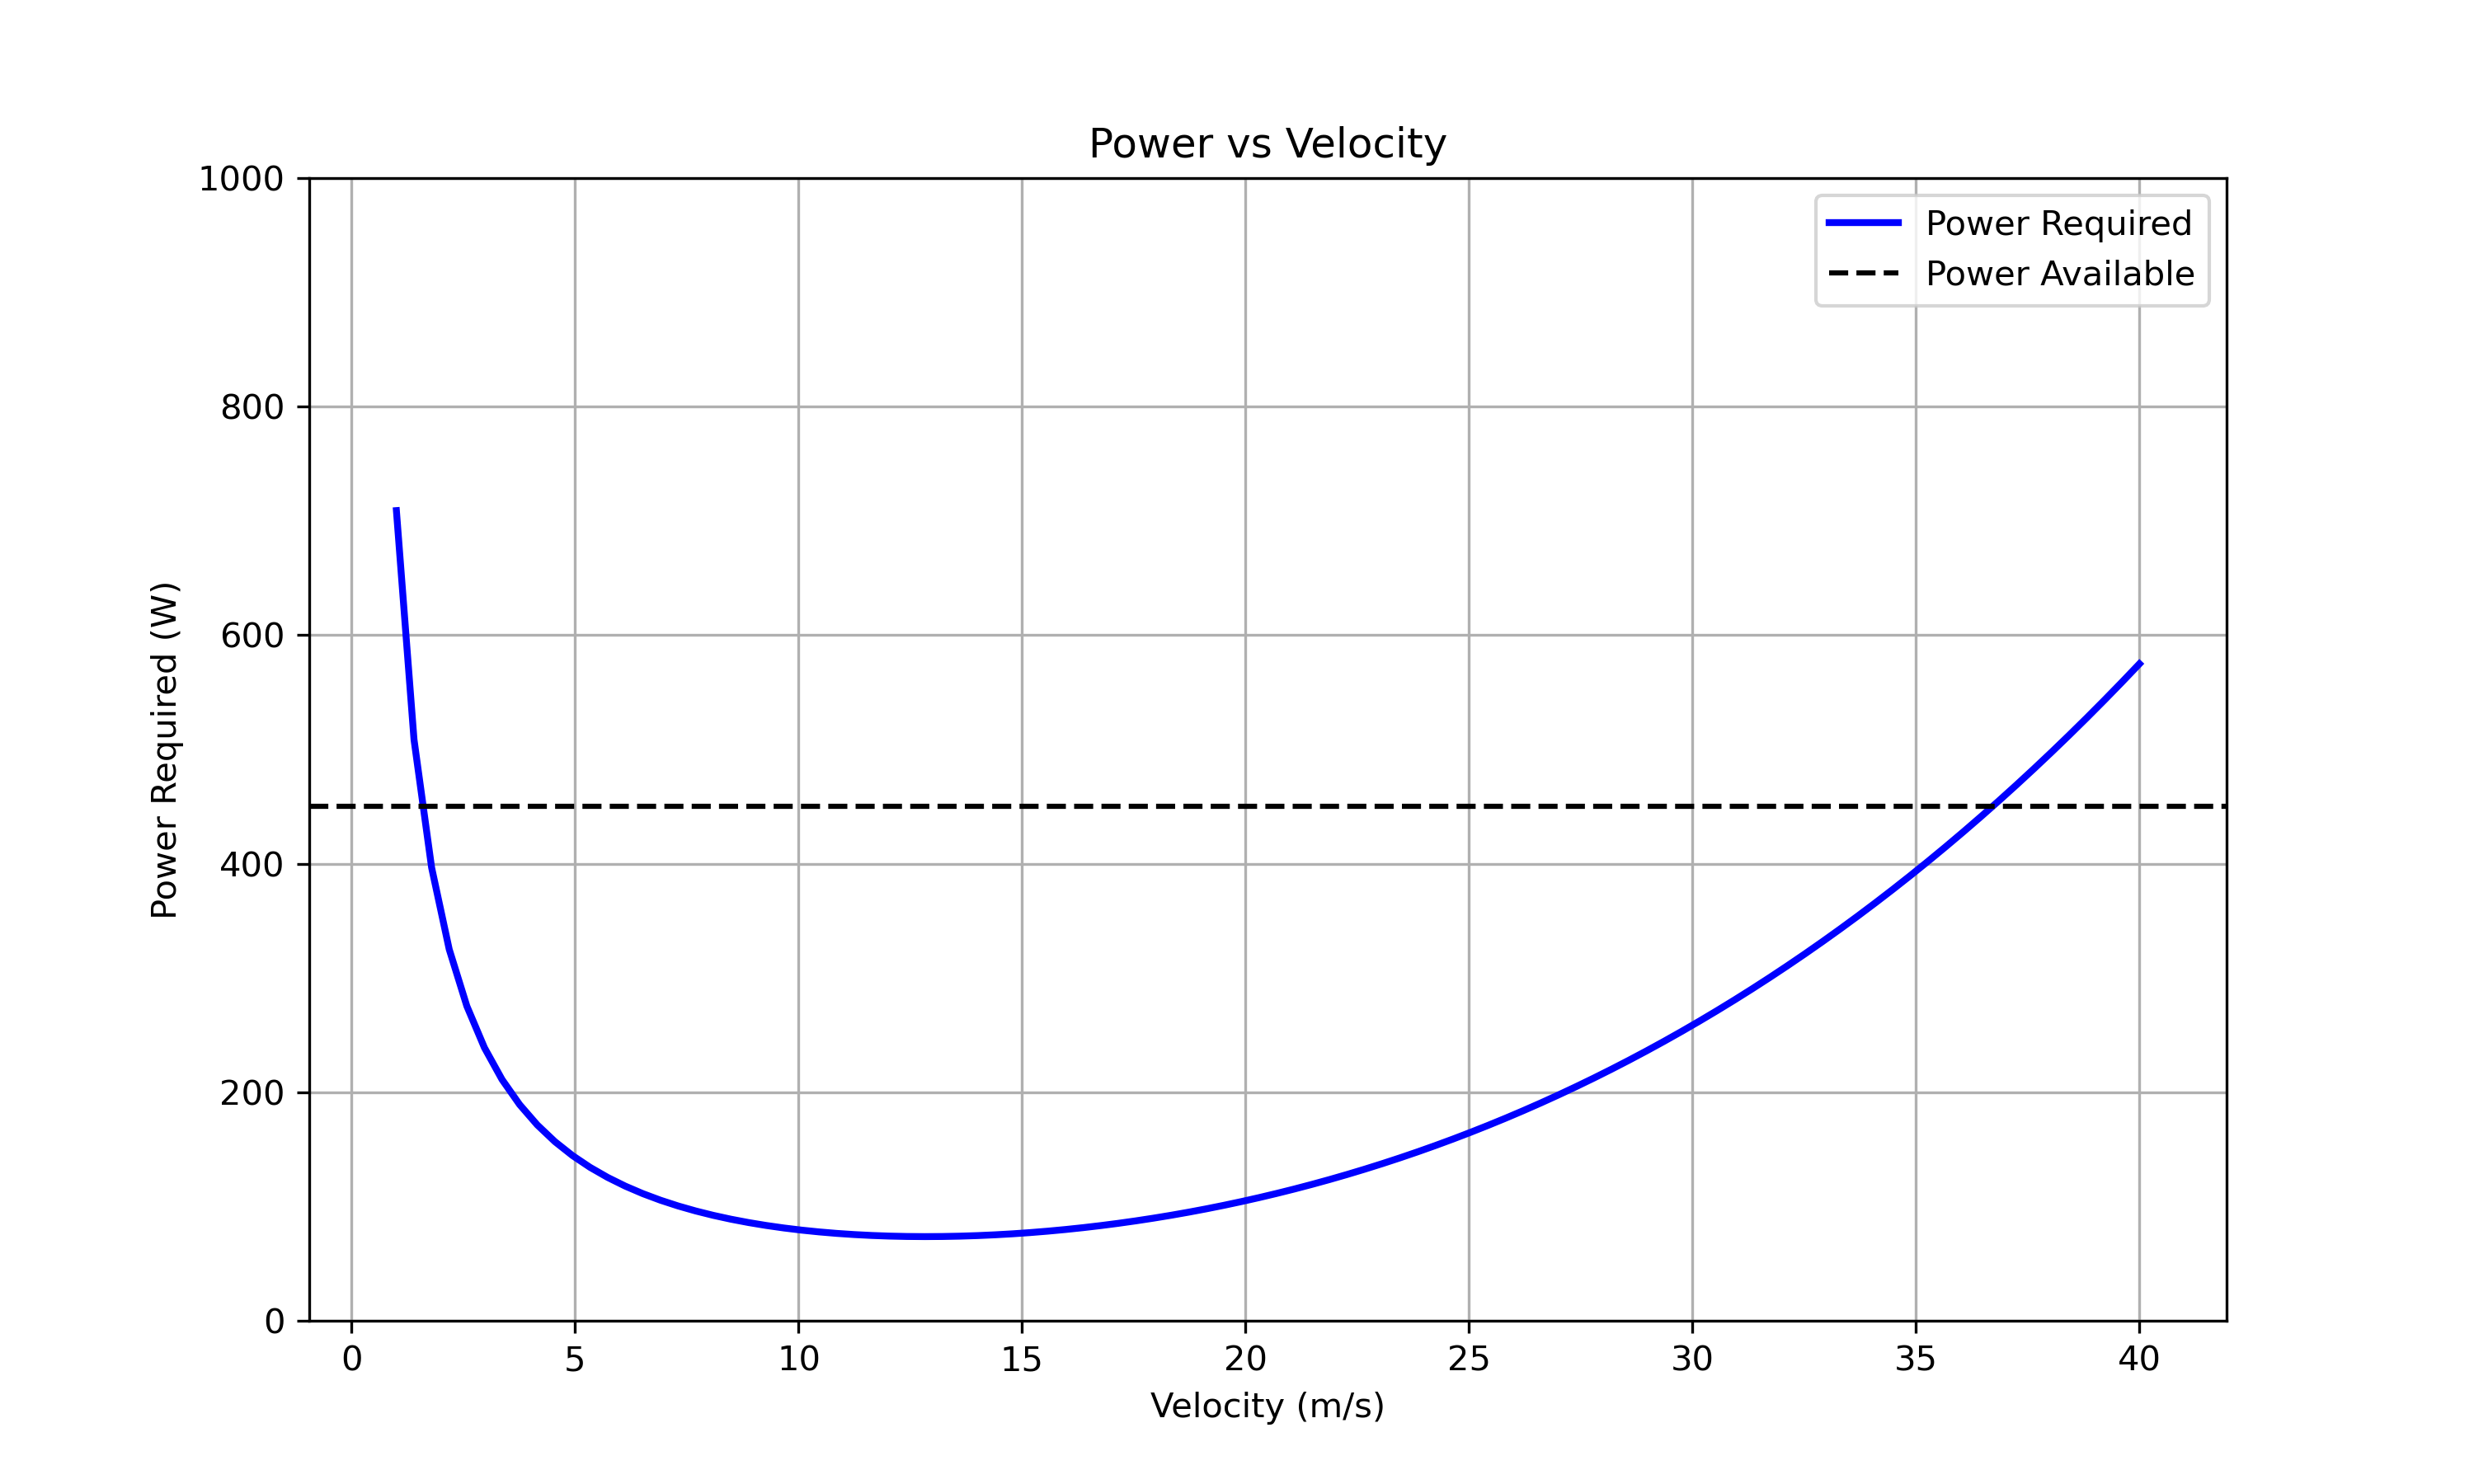
\includegraphics[width=0.5\linewidth]{Power_vs_Velocity.png}
    \caption{Caption}
    \label{fig:placeholder}
\end{figure}

\vspace{0.5cm}
\begin{figure}
    \centering
    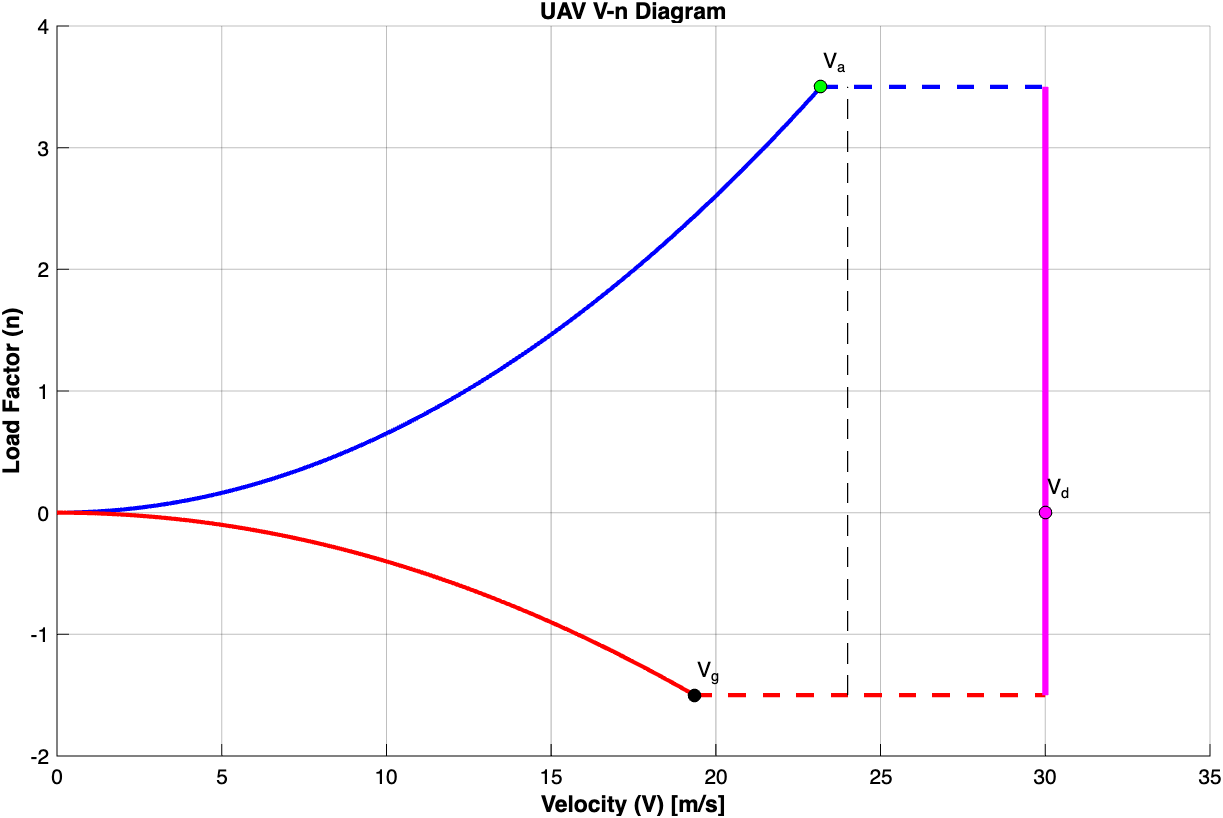
\includegraphics[width=0.5\linewidth]{V_n_before_payload.png}
    \caption{Caption}
    \label{fig:placeholder}
\end{figure}
\end{center}
\end{columns}
\end{frame}

% ============ SLIDE 13: STABILITY 1 ============
\begin{frame}{Stability Analysis (1/2)}

\begin{tikzpicture}[remember picture,overlay]
\fill[lightblue!30] (current page.north west) rectangle ([yshift=-1.2cm]current page.north east);
\end{tikzpicture}

\begin{columns}[T]
\column{0.5\textwidth}
\textbf{\color{navymain}Longitudinal Static Stability:}
\begin{itemize}
\item \textbf{Static margin:} $K_n \approx \textcolor{navydeep}{\textbf{14\%}}$
\item \textbf{Neutral point:} \SI{296}{\milli\meter}
\item \textbf{CG location:} \SI{264}{\milli\meter}
\item \textbf{$C_{m_\alpha}$:} $-0.487$ rad$^{-1}$ (stable)
\item \textbf{$C_{m_0}$:} 0.0125
\end{itemize}

\vspace{0.3cm}
\textbf{\color{navymain}Lateral-Directional:}
\begin{itemize}
\item \textbf{$C_{n_\beta}$:} $+0.0838$ rad$^{-1}$ {\footnotesize(stable)}
\item \textbf{$C_{l_\beta}$:} $-0.0111$ rad$^{-1}$ {\footnotesize(dihedral)}
\item \textbf{$C_{l_p}$:} $-0.659$ rad$^{-1}$ {\footnotesize(roll damp)}
\end{itemize}

\column{0.5\textwidth}
\textbf{\color{navymain}Longitudinal Derivatives:}
\begin{table}
\fontsize{12}{14}\selectfont
\begin{tabular}{@{}lc@{}}
\toprule
\textbf{Derivative} & \textbf{Value} \\
\midrule
$C_{m_q}$ & $-14.94$ rad$^{-1}$ \\
$C_{L_q}$ & $+5.66$ rad$^{-1}$ \\
$C_{D_\alpha}$ & $+0.104$ rad$^{-1}$ \\
$C_{L_M}$ & $+0.023$ \\
\bottomrule
\end{tabular}
\end{table}
\end{columns}
\end{frame}

% ============ SLIDE 14: STABILITY 2 ============
\begin{frame}{Stability Analysis (2/2)}


\textbf{\color{navymain}Dynamic Stability Modes:}

\begin{columns}[T]
\column{0.5\textwidth}
\textit{\color{navydeep}Longitudinal:}
\begin{itemize}
\item \textbf{Short Period:}
  \begin{itemize}
  \item $\omega_n = \SI{7.53}{\radian\per\second}$
  \item $\zeta = \textcolor{navydeep}{\textbf{0.72}}$ (well-damped)
  \item $T = \SI{0.83}{\second}$
  \end{itemize}
\item \textbf{Phugoid:}
  \begin{itemize}
  \item $\omega_n = \SI{0.56}{\radian\per\second}$
  \item $\zeta = 0.074$ (lightly damped)
  \item $T = \SI{11.15}{\second}$
  \end{itemize}
  \begin{figure}
      \centering
      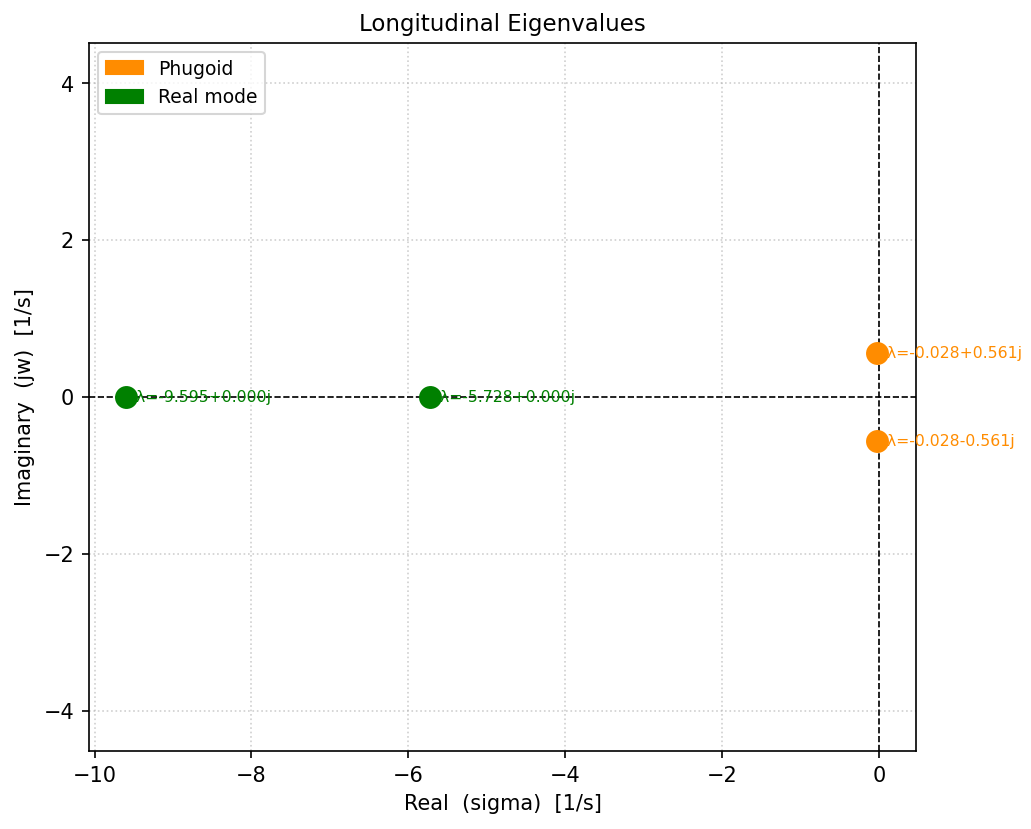
\includegraphics[width=0.5\linewidth]{Longitudinal_eigenvales.png}
      \caption{Caption}
      \label{fig:placeholder}
  \end{figure}
\end{itemize}

\column{0.5\textwidth}
\textit{\color{navydeep}Lateral-Directional:}
\begin{itemize}
\item \textbf{Roll Mode:}
  \begin{itemize}
  \item $\lambda_r = -14.0$ s$^{-1}$
  \item $\tau_r = \SI{0.07}{\second}$
  \end{itemize}
\item \textbf{Dutch Roll:}
  \begin{itemize}
  \item $\omega_n = \SI{5.68}{\radian\per\second}$
  \item $\zeta = 0.348$
  \end{itemize}
\item \textbf{Spiral Mode:}
  \begin{itemize}
  \item $\lambda_s = +0.061$ s$^{-1}$
  \end{itemize}
\end{itemize}
\begin{figure}
    \centering
    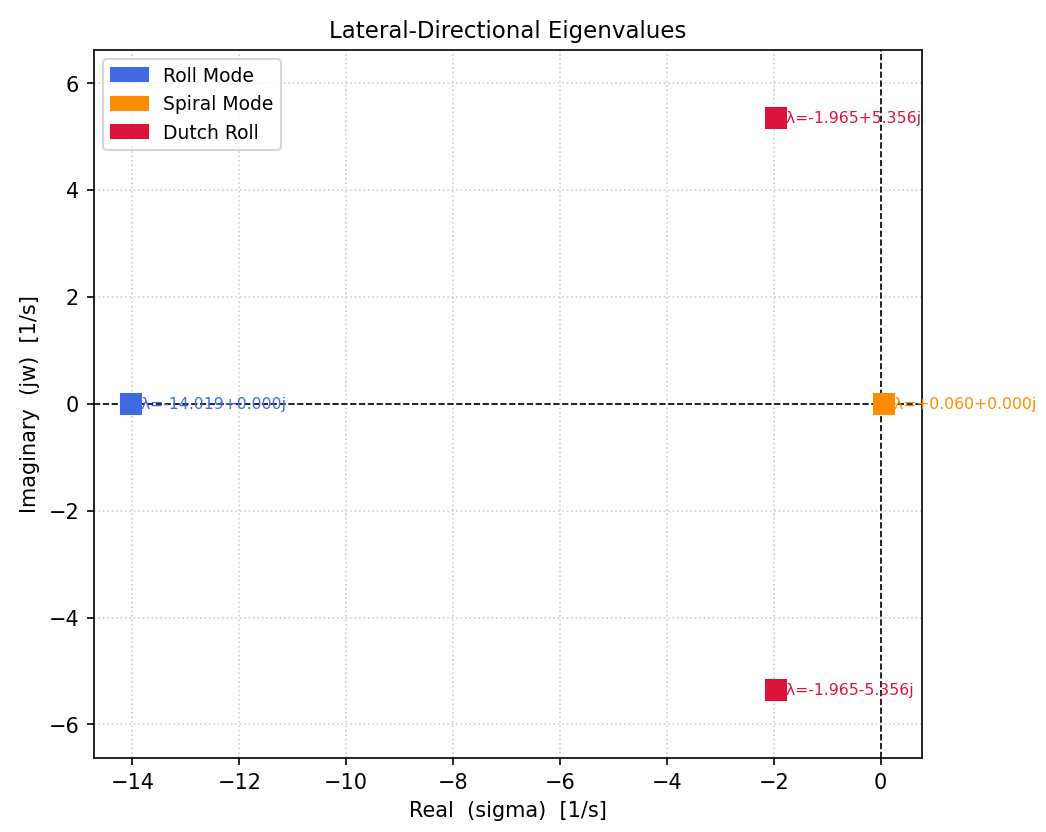
\includegraphics[width=0.5\linewidth]{Lateral_eigenvalues.png}
    \caption{Caption}
    \label{fig:placeholder}
\end{figure}
\end{columns}


\end{frame}

% ============ SLIDE 15: CAD MODEL 1 ============
\begin{frame}{Detailed CAD Model (1/2)}


\textbf{\color{navymain}Physical Configuration:}
\begin{itemize}
\item \textbf{Wing:} High-wing monoplane, rectangular
\item \textbf{Propulsion:} Dual tractor motors on wing leading edge
\item \textbf{Fuselage:} Modular design with quick-swap payload bay
\item \textbf{Empennage:} Conventional tail with T-configuration
\item \textbf{Landing gear:} Tricycle configuration
\item \textbf{Materials:}  carbon fiber spars, Aluminium sheets
\end{itemize}

\vspace{0.3cm}
\textbf{\color{navymain}Design Features:}
\begin{itemize}
\item Central payload drop mechanism with parachute deployment
\item Quick-release battery compartment
\item Integrated avionics bay with telemetry
\item Impact-absorbing landing gear for rough terrain
\end{itemize}
\end{frame}

% ============ SLIDE 16: CAD MODEL 2 ============
\begin{frame}{Detailed CAD Model (2/2)}

\begin{columns}[T]
\column{0.45\textwidth}
\textbf{\color{navymain}Component Integration:}
\begin{itemize}
\item Flight controller \& GPS in nose
\item Battery positioned near nose
\item Payload compartment at CG
\item Motors on wing at 25\% chord
\item 4 servo actuators
\end{itemize}



\column{0.55\textwidth}
\begin{center}
\textbf{\color{navymain}CAD Views:}\\
\vspace{0.15cm}
\colorbox{iceblue}{\parbox{0.9\textwidth}{\centering\small\textcolor{navymain}{\textbf{[Isometric]}}}}\\
\vspace{0.15cm}
\colorbox{iceblue}{\parbox{0.9\textwidth}{\centering\small\textcolor{navymain}{\textbf{[Top view]}}}}\\
\vspace{0.15cm}
\colorbox{iceblue}{\parbox{0.9\textwidth}{\centering\small\textcolor{navymain}{\textbf{[Side view]}}}}\\
\vspace{0.15cm}
\colorbox{iceblue}{\parbox{0.9\textwidth}{\centering\small\textcolor{navymain}{\textbf{[Front view]}}}}
\end{center}
\end{columns}
\end{frame}

% ============ BACKUP SLIDE: REQUIREMENTS COMPLIANCE ============
\begin{frame}{Requirements Compliance Summary}


\begin{table}
\fontsize{13}{15}\selectfont
\begin{tabular}{@{}lcc@{}}
\toprule
\textbf{Requirement} & \textbf{Specification} & \textbf{Achievement} \\
\midrule
Maximum wingspan & \SI{2.00}{\meter} & \textcolor{navydeep}{\textbf{\SI{2.00}{\meter}}} \checkmark \\
Payload capacity & \SIrange{1}{2}{\kilo\gram} & \textcolor{navydeep}{\textbf{\SI{1.20}{\kilo\gram}}} \checkmark \\
Operational radius & \SIrange{40}{50}{\kilo\meter} & \textcolor{navydeep}{\textbf{\SI{41.6}{\kilo\meter}}} \checkmark \\
Total range & \SIrange{80}{100}{\kilo\meter} & \textcolor{navydeep}{\textbf{\SI{83.15}{\kilo\meter}}} \checkmark \\
Endurance & \SIrange{1}{2}{\hour} & \textcolor{navydeep}{\textbf{2 h 5 min}} \checkmark \\
Cruise speed & \SIrange{18}{25}{\meter\per\second} & \textcolor{navydeep}{\textbf{\SIrange{18}{22}{\meter\per\second}}} \checkmark \\
Takeoff distance (STOL) & $< \SI{150}{\meter}$ & \textcolor{navydeep}{\textbf{$< \SI{150}{\meter}$}} \checkmark \\
Static stability & Positive margin & \textcolor{navydeep}{\textbf{14\% MAC}} \checkmark \\
\bottomrule
\end{tabular}
\end{table}

\vspace{0.5cm}
\begin{center}

\begin{tikzpicture}
\fill[navydeep, rounded corners=5pt] (0,0) rectangle (10,1.2);
\node[text=white, font=\Large\bfseries] at (5,0.6) {All Primary Mission Requirements Met};
\end{tikzpicture}
\end{center}
\end{frame}

\end{document}